\documentclass[12pt]{article}

%**********************************************
%* Add additional packages as needed

\usepackage{url,amsmath,setspace,amssymb}
\usepackage{listings}

\usepackage{tcolorbox}
\usepackage{tikz}
\usepackage{xcolor}


\usepackage{color}
\def\R{\color{red}}
\def\B{\color{blue}}

\usepackage{listings}
\usepackage{caption}
\usepackage{float}
\usepackage{graphicx}
\graphicspath{ {./images/} }

\usepackage{hyperref}


%**********************************************
%* Please replace this with your name and your AAU student number
\newcommand{\studentname}{Massimo Calabrigo}
\newcommand{\studentnumber}{12247382}



%**********************************************
%* Some more or less useful stuff, add custom stuff as needed

\lstnewenvironment{myalgorithm}[1][] %defines the algorithm listing environment
{
   % \captionsetup{labelformat=algocaption,labelsep=colon}
    \lstset{ %this is the stype
        mathescape=true,
        frame=none,
        numbers=none,
        basicstyle=\normalsize,
        keywordstyle=\color{black}\bfseries\em,
        keywords={,input, output, return, datatype, function, in, if, else, foreach, while, begin, end, },
        numbers=left,
        xleftmargin=.04\textwidth,
        #1 % this is to add specific settings to an usage of this environment (for instance, the caption and referable label)
    }
}
{}


\newtcolorbox{alert}[1]{
colback=red!5!white, colframe=red!75!white,fonttitle=\bfseries, title = #1}

\newtcolorbox{commentbox}[1]{
colback=black!5!white, colframe=black!75!white,fonttitle=\bfseries, title = #1}



%**********************************************
%* Leave the page configuration as is
\setlength{\oddsidemargin}{.25in}
\setlength{\evensidemargin}{.25in}
\setlength{\textwidth}{6.25in}
\setlength{\topmargin}{-0.4in}
\setlength{\textheight}{8.5in}

\newcommand{\heading}[5]{
\renewcommand{\thepage}{#1-\arabic{page}}
\noindent
\begin{center}
	\framebox[\textwidth]{
	\begin{minipage}{0.9\textwidth} \onehalfspacing
	{\bf 622.755 -- \unitname} \hfill #2

	{\centering \Large #5

	}\medskip
	{#3 \hfill #4}
	\end{minipage}
}
\end{center}
}

\newcommand{\unitname}{Introduction to Cybersecurity}
\newcommand{\maxpages}{5}
\newcommand{\handout}[3]{\heading{#1}{#2}{\studentname}{\studentnumber}{#3}}

%**********************************************
%* The document starts here
\begin{document}
\handout{\maxpages}{Summer Term, 2022/23}{Project Write Up}

\tableofcontents
\section{Introduction}
Nowadays cryptography is fast becoming more and more present in the life of the public.\\
Cryptography allows secure HTTP connections through TLS/SSL\cite{TLS}, End to End encryption \cite{crypto_application}, blockchain technology \cite{blockchain}, Multi Party Computation and many more applications \cite{crypto_application}.
\\
In this work we are going to look at Multi Party Computation (MPC), a branch of cryptography regarding the computation of a shared output between a set of parties, without any party knowing any of the inputs of the others.
 Specifically we are going to explore two practical use cases of this technology: Double auctions\cite{sealed_bid:wikipedia} and Genetic Testing \cite{genetic_testing}.\\
\\
In section 2 we will briefly introduce a MPC solution applied to a double auction.\\
\\
In section 3 we will see applications of specific MPC solutions: Yao circuits and Homorphic Encryption, used in the context of Generic Testing, a technique used to analyze DNA, while discussing the social and legal implications of Genetic Testing with and without MPC.\\

\section{Danish Sugar Beet Auction}
In January 2008 the Danish company "Danisco", which processes Sugar Beets, needed to find the new market price for Sugar Beets due to reduced subsidies from the European Union and lowered prices, and thought to organize an auction in which both the producers and Danisco would state their desidered prices, and a new market price would be computed \cite{sealed_bid:wikipedia}.\\
\\
 The fact that Danisco knew the offers of each producer was a problem though. If Danisco had this information, then it could have learned about the financial situation of every producer, and use these informations against them, 
 so, to solve this problem, Danisco proposed a double auction, that is an auction in which buyers and sellers can propose some price $p_i$, and then, based on a set of $p_i$ values from both buyers and seller, a market price $p$ would be computed.\\
 To achieve privacy of the offers in the auction MPC was employed, in this way the market price was computed without Danisco knowing the market price proposal of any producer, while everyone having access to the new shared market price.\\
 \\
 The MPC solution to the Danish Sugar Beet Auction was advantageous to every party: Danisco ensured that the offers from the producers were honest, and the market price fair, and producers ensured that their offer was secret, and couldn't be used against them by Danisco.

\newpage
\section{DNA and Genetic Testing}
\label{sec:section_3}
DNA is a chemical structure, composed of 4 "nucleotides": A,C,T,G , which defines many characteristic of a person, and influences many more.\\
From DNA, with a set of techniques called Genetic Testing, it is possible to extract informations like predisposal toward good mental health \cite{nature:mental_health}, auto-immune conditions \cite{nature:autoimmune}, and even specific personality traits \cite{genetic_personality}. 
\subsection{DNA: privacy concerns}
Since DNA is the ultimate source of personal information,
sharing of this data is particularly dangerous. DNA can reveal
information about disease susceptibility and ancestry not only
of the individual but of his or her extended family. Disclosure
of this information could result in discrimination by insurance
companies or reveal unnecessarily intimate information about
an individual or even a family member \cite{genetic_testing}; for these reasons 
a person should not make public its DNA.

\subsection{Extract information from DNA: Genetic Testing}
Genetic Testing is a set of techniques performed on a genome, which aims to predict predisposal toward specific diseases or genetic traits, by searching for certain matching subsequences in the genome, breaking the DNA into fragments, using subsequences, and measure their length, finding mismatches in specific positions of the subsequences, $\dots$
\subsubsection{Privacy and Social aspects}
If a medical provider wants to perform Genetic Testing on a customer DNA, then the customer should trust the medical provider not to make the DNA public. Even if it's legally feasible to make a contract such that the medical provider won't make the genome public, and many genome sequence companies have such privacy policy \cite{veritas_privacy}, it could always happen that the customer genome leaks out anyway by hacking, or the company may be sold and the privacy contract would be changed.\\
In the end the customer has to trust the company, and even if the company has interest in not disappointing this trust, there may be out of control conditions, such as the ones listed earlier, in which data leaks out anyway, and once it happens, all sort of informations of the customer become available \ref{sec:section_3}.
\subsubsection{Legal aspects}
In the USA, which is currently the largest market in DNA sequencing, the only law protecting DNA privacy is the Genetic Information Non-discrimination Act (GINA) \cite{GINA}, which is a 25 years old law which barring employers and insurance companies access to DNA data, but does nothing to impede a large big data DNA market, which could be exploited by big companies to better classify their users.\\
There is much space for legislation in this field not only in the USA, but also in the rest of the world.
\subsection{Genetic Testing and Multi Party Computation}
For the aformentioned privacy problems, Genetic Testing requires to do computations on the genome, without knowing it in clear, and this can be achieved by Multi Party Computation.\\
Various Multi Party Computation solutions have been studied for application in the Genetic Testing problem \cite{genetic_testing}:
\begin{itemize}
    \item Yao's Garbled Circuits for the \textbf{Edit Distance}, a measure of similarity between subsequences, that is the minimum number of insertions, deletions, and substitutions needed to convert the subsequence $a$ into the subsequence $b$
    \item Homomorphic Encryption for \textbf{Disease susceptibility}
\end{itemize}
The result of the application of MPC to Genetic Testing is that with one MPC technique or the other, all the Genetic Testing techniques can be applied (see figure \ref{fig:table}) with reasonable efficiency \cite{genetic_testing}, while mantaining both the customer genome and the company specific subsequences private.\\
\begin{figure}[H]
    \centering
    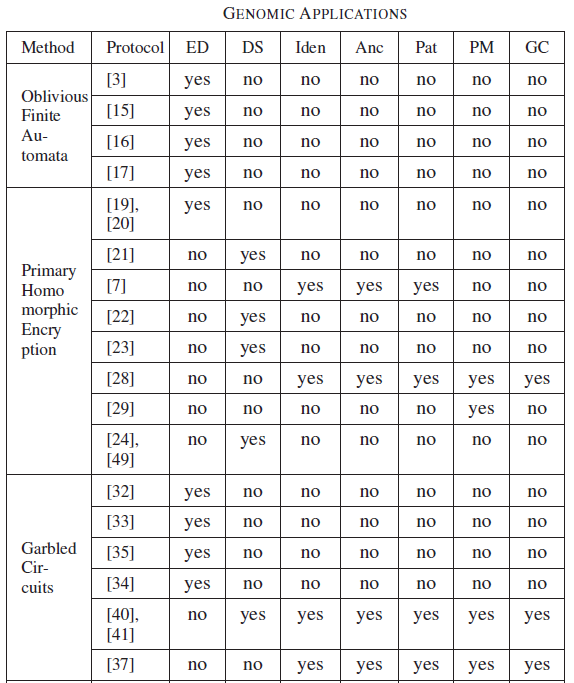
\includegraphics[width=0.4\textwidth]{table}
    \caption{ED: Edit Distance, DS: Disease Susceptibility, protocol column defines specific implementations of MPC, method column defines different types of MPC, while the remaining columns contains Genetic Testing techniques we didn't cover in this paper. We can see that both Edit Distance and Disease Susceptibility are covered by some MPC technique \cite{genetic_testing}}
    \label{fig:table}
\end{figure}
\newpage
\section{Conclusions}
We saw two main applications of Multi Party Computation: MPC applied to the Sugar Beet Auction protected the privacy of the customers, and impeded the company "Danisco" to exploit the offer proposals to infer their financial situations, while 
MPC applied to Genetic Testing enabled both the customer to not revealing his genome, and the medical provider not revealing for which specific subsequences it tested the genome with, hence protecting both the privacy of the customer, and the privacy of the medical provider.\\
\\
MPC shows itself as a promising and effective technique in all that cases where an output must be computed without the parties knowing the inputs of the other parties, and without needing to trust a central authority.\\
In the case of Genetic Testing MPC solves the problem of trusting DNA to a company, hence, in order to ensure DNA privacy, it should become standard for medical providers and DNA sequencing companies to use this technique.


\begin{thebibliography}{10}
\bibitem{genetic_testing}
A Survey of Secure Multiparty Computation Protocols for Privacy Preserving Genetic Tests, 
\newblock {\em IEEE First International Conference on Connected Health: Applications, Systems and Engineering Technologies}, 2016.
\bibitem{nature:autoimmune}
\href{https://www.nature.com/articles/d41586-021-01839-6}{Cracking the genetic code of autoimmune disease}
\bibitem{nature:mental_health}
\href{https://www.nimh.nih.gov/health/publications/looking-at-my-genes}{Looking at My Genes: What Can They Tell Me About My Mental Health?}
\bibitem{genetic_personality}
\href{https://pubmed.ncbi.nlm.nih.gov/29152902/}{The genetics of human personality}
\newblock {\em ICISC}, 2003.
\bibitem{sealed_bid:wikipedia}
\href{https://en.wikipedia.org/wiki/Danish_Sugar_Beet_Auction}{Danish Sugar Beet Auction}
\bibitem{crypto_application}
\href{https://resources.infosecinstitute.com/topic/how-is-cryptography-used-in-applications/}{How Is Cryptography Used In Applications?}
\bibitem{GINA}
\href{https://www.genome.gov/about-genomics/policy-issues/Genetic-Discrimination}{Genetic Information Non-discrimination Act}
\bibitem{TLS}
\href{https://it.wikipedia.org/wiki/Transport_Layer_Security}{Transport Layer Security}
\bibitem{blockchain}
\href{https://it.wikipedia.org/wiki/Blockchain}{Blockchain}
\bibitem{veritas_privacy}
\href{https://veritas.azureedge.net/cdn/website/2023/01/63ca8df50b7a5-63ca8df50b7a6Veritas-Genetics-Privacy-Notice.pdf.pdf}{Vertitas Privacy Policy}
\end{thebibliography}

\end{document}



